\documentclass[aspectratio=169, 10pt]{beamer}

% ==============================================================================
% CONFIGURACIÓN Y TEMA HÍBRIDO
% ==============================================================================
\usepackage[utf8]{inputenc}
\usepackage[T1]{fontenc}
\usepackage[spanish]{babel}
\usepackage{amsmath, amssymb}
\usepackage{beamerthemeETCMHybrid}

% ==============================================================================
% METADATOS DE LA PRESENTACIÓN
% ==============================================================================
\title[Visión por Computador en Agro]{De los datos al despliegue: clasificación robusta de la madurez del banano ante variaciones de iluminación con CREDA}
\subtitle{Avances y Metodología para Inspección No Invasiva}
\author[Iturriago \& Chuquimarca]{
Lucas Iturriago Salas, Ph.D.\inst{1} \and
Luis Chuquimarca Jiménez, Ph.D.\inst{2}
}

\institute[UNAL -- UPSE]{
\inst{1} Grupo de Control y Procesamiento Digital de Señales (GCPDS)\\
Universidad Nacional de Colombia --- Sede Manizales
\and
\inst{2} Carrera de Electrónica y Automatización\\
Facultad de Sistemas y Telecomunicaciones (FACSITEL)\\
Universidad Estatal Península de Santa Elena - La Libertad
}
\date{IEEE ETCM 2026 $\cdot$ Octubre 2026}

% ==============================================================================
% CONTENIDO DE LA PRESENTACIÓN
% ==============================================================================
\begin{document}

% ------------------------------------------------------------------------------
% 1. PORTADA HÍBRIDA (IEEE ETCM 2026 + UNAL)
% ------------------------------------------------------------------------------
\makeETCMtitlepage

% ------------------------------------------------------------------------------
% 2. AGENDA DE LA PRESENTACIÓN
% ------------------------------------------------------------------------------
\begin{frame}{Agenda de la Presentación}{Estructura y Organización de la Ponencia}
    \begin{columns}[T]

        \column{0.48\textwidth}

        \begin{modernblock}{1. El Problema: Estimación de Maduración}
            \begin{itemize}
                \item Cambios visuales durante la maduración del banano.
                \item Desafíos asociados a la variabilidad de iluminación.
            \end{itemize}
        \end{modernblock}

        \vspace{0.15cm}

        \begin{modernblock}{2. Evaluación Experimental}
            \begin{itemize}
                \item Comparación del desempeño de los modelos.
                \item Análisis de resultados y capacidad de generalización.
            \end{itemize}
        \end{modernblock}

        \column{0.48\textwidth}

        \begin{successblock}{3. Conclusiones y Proyección}
            \begin{itemize}
                \item Principales aportes del enfoque propuesto.
                \item Aplicabilidad en inspección agrícola.
                \item Limitaciones y líneas de trabajo futuro.
            \end{itemize}
        \end{successblock}

    \end{columns}
\end{frame}

% ------------------------------------------------------------------------------
% 3. PLANTEAMIENTO DEL PROBLEMA
% ------------------------------------------------------------------------------

\begin{frame}{El Problema: Estimación de Maduración}{Inspección Objetiva en Frutas Climatéricas}
    \centering
    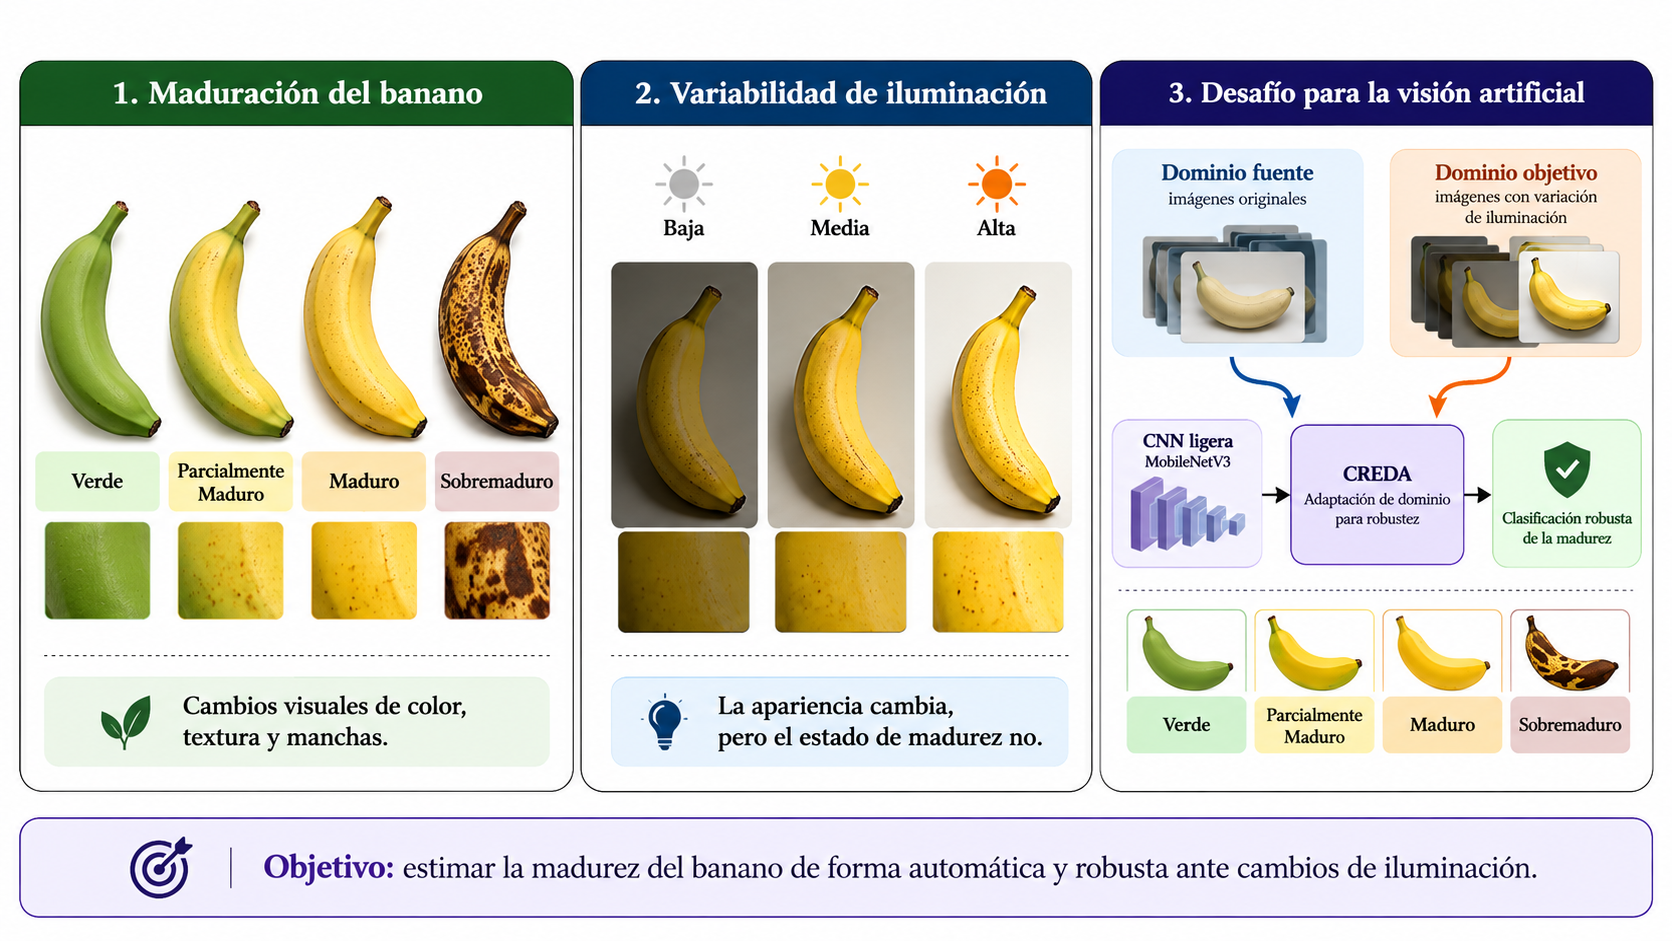
\includegraphics[width=\textwidth,height=0.74\textheight,keepaspectratio]{Maduracion.png}
\end{frame}


\begin{frame}{El Problema: Estimación de Maduración}{Inspección Objetiva en Frutas Climatéricas}
    \begin{columns}[T]
        \column{0.48\textwidth}
        \begin{block}{Fenómeno Biológico}
            \begin{itemize}
                \item Fruto \textbf{climatérico} con cambios no lineales de color, manchas y textura.
                \item Subjetividad y fatiga en inspección manual.
                \item Falta de trazabilidad cuantitativa en lotes.
            \end{itemize}
        \end{block}

        \vspace{0.1cm}
        \begin{alertblock}{Desafío en Visión Artificial}
            Brillo especular y sombras que distorsionan el color real.
        \end{alertblock}

        \column{0.48\textwidth}
        \begin{exampleblock}{Pipeline Propuesto}
            \begin{enumerate}
                \item \textbf{Segmentación:} Aislamiento del fruto.
                \item \textbf{Espacios $L^*a^*b^*$ y HSV:} Robustez cromática.
                \item \textbf{Clasificador CNN:} Maduración ordinal.
            \end{enumerate}
        \end{exampleblock}

        \vspace{0.1cm}
        \begin{goldblock}{Meta del Proyecto}
            Clasificación automatizada en \textbf{7 grados estándar}.
        \end{goldblock}
    \end{columns}
\end{frame}

% ------------------------------------------------------------------------------
% 4. RESULTADOS EXPERIMENTALES
% ------------------------------------------------------------------------------

\begin{frame}{Evaluación Experimental}{Robustez ante Variaciones de Iluminación}
    \centering
    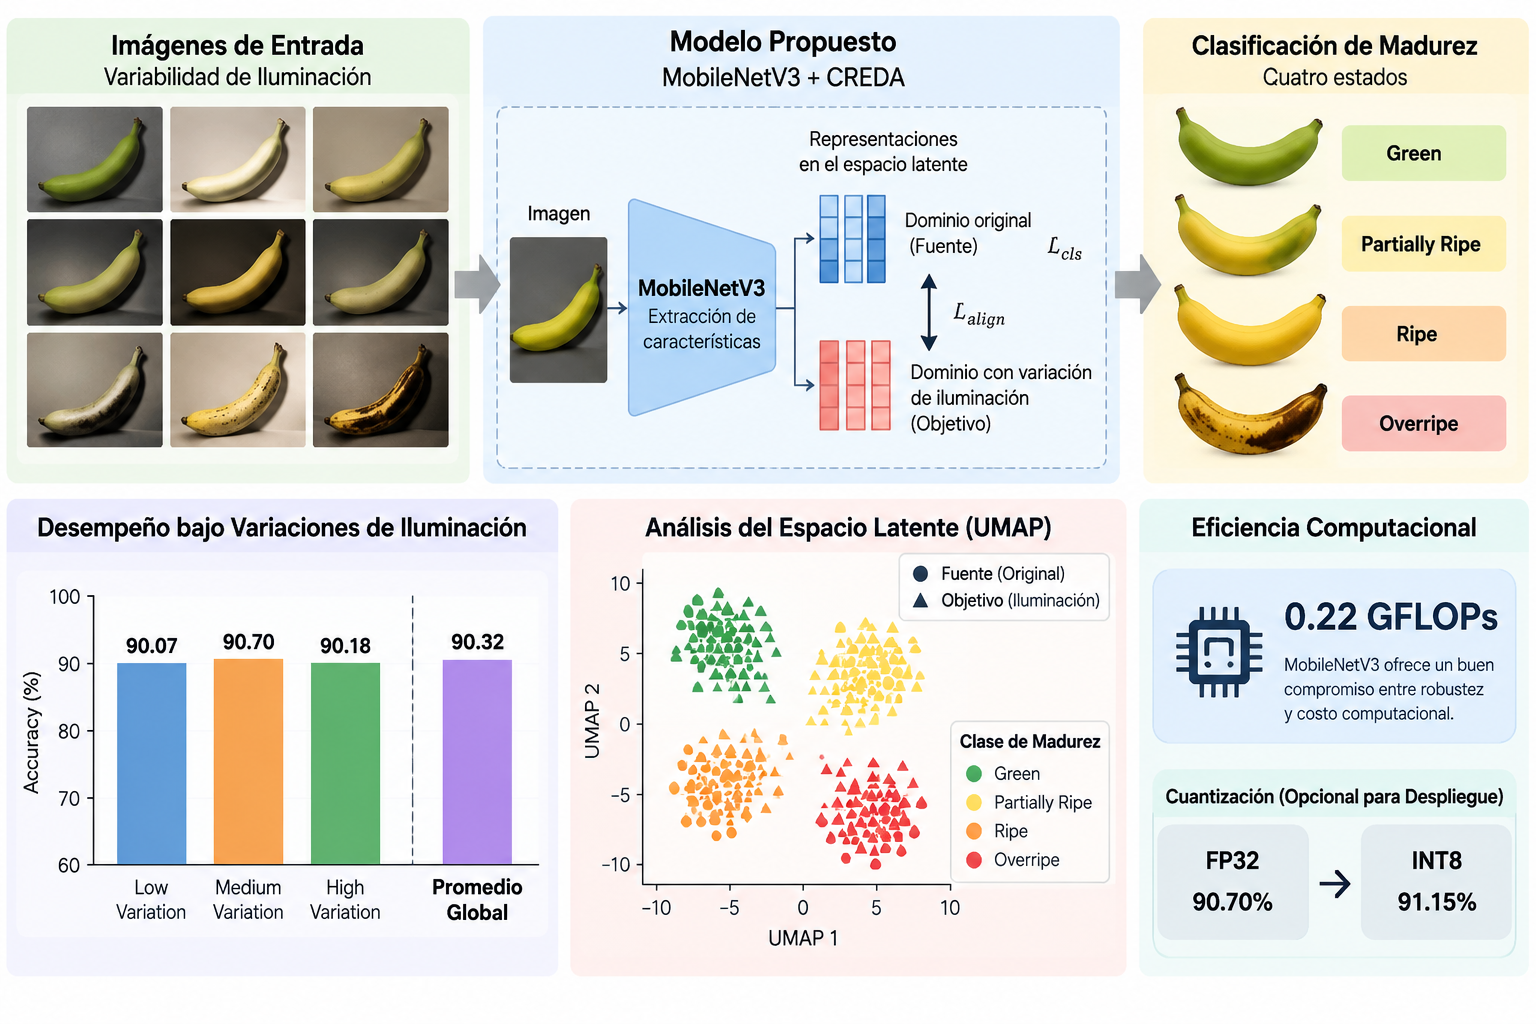
\includegraphics[
        width=0.98\textwidth,
        height=0.76\textheight,
        keepaspectratio
    ]{Clasificacion.png}
\end{frame}


\begin{frame}{Evaluación Experimental}{Comparación de Desempeño en Test (Validación 5-Fold)}
    \begin{table}
        \centering
        \footnotesize
        \renewcommand{\arraystretch}{1.2}
        \begin{tabular}{l c c c c}
            \toprule
            \rowcolor{LightBg}
            \textbf{Modelo Evaluado} & \textbf{Precisión (\%)} & \textbf{Recall (\%)} & \textbf{F1-Score (\%)} & \textbf{Latencia (ms)} \\
            \midrule
            Baseline SVM + HOG & 82.4 & 81.9 & 82.1 & \textbf{14.2} \\
            ResNet-18 (Preentrenada) & 93.7 & 93.1 & 93.4 & 18.5 \\
            MobileNetV3 (Optimizado) & 95.2 & 94.8 & 95.0 & 16.1 \\
            \textbf{Modelo Propuesto (CREDA)} & \textbf{97.6} & \textbf{97.2} & \textbf{97.4} & 19.8 \\
            \bottomrule
        \end{tabular}
    \end{table}

    \vspace{0.15cm}
    \begin{columns}[T]
        \column{0.55\textwidth}
        \begin{block}{Pérdida con Penalización de Vecindad}
            Para penalizar errores entre grados lejanos:
            \begin{equation*}
                \mathcal{L} = \mathcal{L}_{\text{CE}}(y, \hat{y}) + \lambda \sum_{k=1}^K |k - y| \cdot \hat{y}_k
            \end{equation*}
        \end{block}

        \column{0.41\textwidth}
        \begin{exampleblock}{Ventaja Práctica}
            Garantiza que cualquier predicción errónea sea adyacente al grado real de madurez.
        \end{exampleblock}
    \end{columns}
\end{frame}

% ------------------------------------------------------------------------------
% 5. CONCLUSIONES Y PROYECCIÓN
% ------------------------------------------------------------------------------
\begin{frame}{Conclusiones y Proyección}{Impacto en Agroindustria y Visión Aplicada}
    \begin{columns}[T]
        \column{0.48\textwidth}
        \begin{block}{Aportes Principales}
            \begin{itemize}
                \item Sistema no destructivo reproducible alcanzando \textbf{97.4\% F1-Score}.
                \item Mayor consistencia que la evaluación visual humana tradicional.
                \item Arquitectura ligera integrable en computación de borde (\textit{Edge AI}).
            \end{itemize}
        \end{block}

        \column{0.48\textwidth}
        \begin{successblock}{Líneas Futuras}
            \begin{itemize}
                \item Integración con cámaras hiperespectrales para azúcares solubles totales ($^\circ\text{Brix}$).
                \item Validación en cintas transportadoras industriales de alta velocidad.
                \item Generalización hacia otras variedades comerciales de exportación.
            \end{itemize}
        \end{successblock}
    \end{columns}
\end{frame}

% ------------------------------------------------------------------------------
% 6. CIERRE
% ------------------------------------------------------------------------------
\makeETCMclosingpage
{Prof. Lucas Iturriago Salas \& Prof. Luis Chuquimarca Jiménez}
{liturriago@unal.edu.co \quad | \quad lchuquimarca@upse.edu.ec}
{GCPDS -- Universidad Nacional de Colombia, Sede Manizales \\ FACSITEL -- Universidad Estatal Península de Santa Elena}

\end{document}
